\chapter{REFERENCIAL TEÓRICO }

\section{Mercado Financeiro}
Muitos conceitos que serão utilizados neste trabalho são referentes ao mercado financeiro, portanto para sintonizar os leitores, nesta secção será apresentada uma breve descrição dos conceitos referentes ao mercado financeiro.

\subsection{Bolsa de valores}
A bolsa de valores é um ponto comum onde as empresas podem negociar suas ações. Todos os países que possuem empresas de capital aberto possuem uma bolsa de valores, no Brasil este ponto de compra e venda de ações é chamado de Bovespa. A Bovespa é a única regulamentada no Brasil\cite{EQUIPETORORADAR}. Abaixo na Figura 1 pode-se ver as principais bolsas de valores até o momento.

 \begin{figure}[htb]
 \centering
 	\caption{Principais bolsas de valores}
 	\label{fig:principais-bolsas}
 	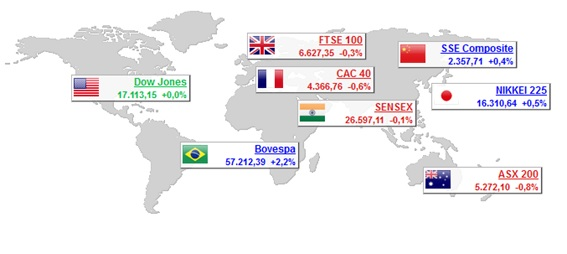
\includegraphics[scale=0.8]{figuras/principais-bolsas.jpg}
 	\fonte{https://br.advfn.com/mundo}
 \end{figure}
 
 A Figura 1 acima também indica o índice de cada bolsa de valores ali representada. O índice da bolsa é dado pelo desempenho de compra e venda de ações negociadas dentro da bolsa em questão, e indica o desempenho médio do mercado acionário de cada país\cite{IBOVESPA}.

\subsection{Preços}
Geralmente a forma mais comum de se analisar o desempenho dos preços de uma ação é o valor de fechamento, esta é a forma que a mídia usa para fazer a divulgação, porém existem muitas variações do preço da ação ao longo do dia. Para se estabelecer um preço para uma determinada ação baseia-se a lei da oferta e da procura, quanto mais compras uma determinada ação ter maior será seu valor, também pode ser usado como métrica a perspectiva de crescimento da empresa\cite{CITI}.  Quando se busca os dados históricos acerca dos preços de uma ação será encontrado estes dados usando diferentes métricas, o site da Bovespa e do yahoo finance disponibilizam as seguintes métricas:

 \begin{itemize}
	\item Abertura - É o valor da ação no momento da abertura do pregão.
    \item Máximo - Indica o valor mais alto que a ação atingiu durante o dia. Esta é uma métrica muito interessante para saber qual é a tendência da ação, pois se o valor máximo for muito maior que o valor de fechamento indica que houve queda no preço da ação e a tendência é que continue caindo. Se o valor máximo for muito próximo do valor de fechamento indica uma tendência de alta.
    \item Mínimo - Indica o menor valor que a ação teve no período. A interpretação é ao máximo.
    Fechamento - Indica o valor da ação no final do pregão. É a métrica mais comumente utilizada pela mídia para a divulgação dos preços de ações.
    \item Fechamento Ajustado - É o valor de fechamento após o cálculo e distribuição dos dividendos.
    \item Volume - Indica quantas ações foram negociadas no período.
\end{itemize}

\section{Série Temporal}
“A classe de fenômenos cujo processo observacional e consequente quantificação numérica gera uma sequencia de dados distribuídos no tempo é denominada série temporal” \cite{MUELLER}, portanto uma série temporal é a variação de um valor ao longo do tempo. Este valor pode variar apenas em função do tempo eu em função de um conjunto de variáveis, desde que seja em função do tempo\cite{AMADOR}, ou como \citeonline[]{PEDROSO} define série Temporal é uma realização ou trajetória de um processo estocástico. Pode-se citar como exemplo de séries temporais as temperaturas máximas e mínimas diária da cidade de Videira, a variação do preço do dólar ou a variação do preço de uma ação. Abaixo na Figura 2 temos uma representação de uma série temporal das ações de uma empresa qualquer.

\begin{figure}[htb]
 \centering
 	\caption{Série temporal}
 	\label{fig:Série temporal}
 	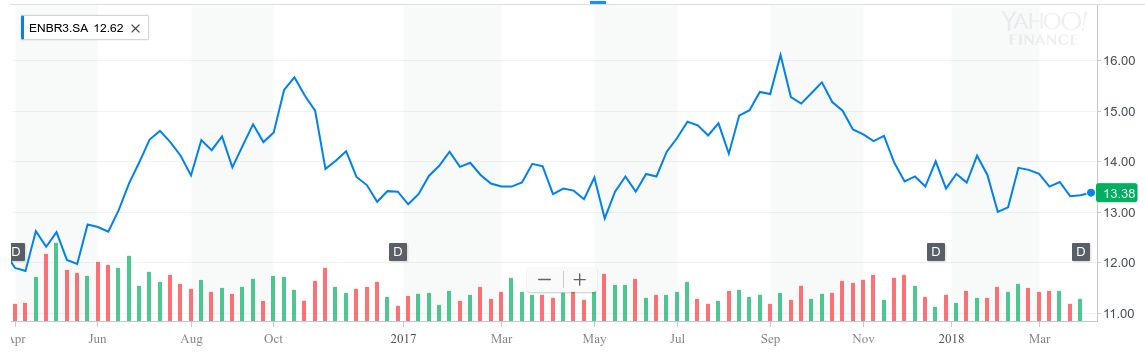
\includegraphics[scale=0.5]{figuras/serie-temporal-yahoo.png}
 	\fonte{Adaptada de https://finance.yahoo.com}
 \end{figure}

Na Figura 2 pode-se perceber que os valores da ação desta empresa tendem a ter valores próximos em determinados meses do ano. As variações sempre seguem um padrão, e com o uso de redes neurais artificiais pode-se identificar este padrão e tentar chegar em um valor aproximado da ação.

\section{Inteligência Artificial}
Desde os primórdios da humanidade nós tentamos compreender o que é a inteligência humana, como que um mero humano, que nada mais é que um simples pedaço de matéria, consegue compreender e modificar um universo muito maior. O campo da inteligência artificial ou IA, tenta compreender e reproduzir a inteligência humana em máquinas \cite{RUSSUEL}. 

A IA é um campo relativamente novo, os trabalhos relacionados ao desenvolvimento desta ciência começaram logo após a segunda guerra mundial e o nome desta nova subárea da ciência foi criado em meados de 1956.

Para definir Inteligência artificial é necessário quebrar o termo, dessa forma teremos os termos “Inteligência” e “Artificial”, desta forma podemos dizer que “artificial” é tudo aquilo feito pelo homem \cite{ROSA}. Para definir o termo “inteligência” é um pouco mais difícil, para isso precisamos recorrer a filosofia e psicologia, se olharmos no dicionário inteligência é a capacidade de compreender e resolver novos problemas e conflitos e de adaptar-se a novas situações. Uma boa definição para IA é, segundo Winston (1992), “O estudo de computações que tornem possível perceber e agir”.

\subsection{Redes Neurais Artificiais}
As redes neurais artificiais (RNA’s) são sistemas paralelos distribuídos compostos por unidades de processamento simples (neurônios artificiais) que calculam determinadas funções matemáticas, seu objetivo é imitar o comportamento do cérebro biológico, porém possuem um número muito inferior de neurônios, estes neurônios podem processar inúmeras variáveis ao mesmo tempo. O grande diferencial das RNA’s para outros sistemas é a capacidade de interpretar o meio externo e se adaptar a ele \cite{FINOCCHIO} \cite{BRAGA}.

\subsubsection{Neurônio artificial}
O neurônio artificial é uma estrutura muito simples inspirada no neurônio biológico. Da mesma forma que um neurônio biológico tem os dendritos responsáveis por receber os impulsos elétricos e conduzi-los até o corpo celular e o axônio encarregado de enviar a saída até o dendrito do próximo neurônio (Figura 3), o neurônio artificial é composto por várias entradas (dendritos) que recebem os valores x1, x2, x3, …, xn correspondentes as ativações dos neurônios anteriores, possui também um terminal de saída y que representa o axônio do neurônio biológico. Cada entrada entrada do neurônio artificial possui um peso, chamado de peso sináptico, dado por w, os pesos servem para o neurônio artificial identificar o grau de relevância daquela entrada \cite{BRAGA}. O neurônio artificial está representado na Figura 4.

\begin{figure}[htb]
 \centering
 	\caption{Neurônio Biológico}
 	\label{fig:Neurônio Biológico}
 	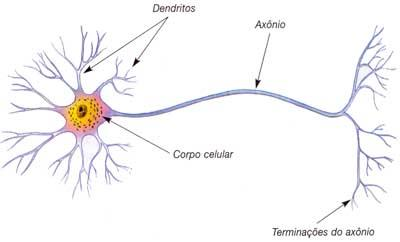
\includegraphics[scale=1.8]{figuras/neuronio-biologico.jpg}
 	\fonte{www.researchgate.net}
 \end{figure}
 
\begin{figure}[htb]
 \centering
 	\caption{Neurônio Artificial}
 	\label{fig:Neurônio Artificial}
 	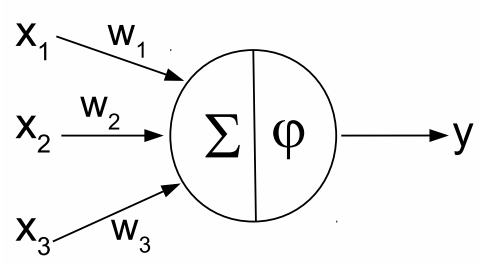
\includegraphics[scale=0.9]{figuras/neuronio-artificial.png}
 	\fonte{\cite{GIACOMELL}.}
 \end{figure}
 
 \subsubsection{Função de ativação}
 A função de ativação é responsável por gerar a saída do neurônio a partir da somatória das entradas com seus respectivos pesos. Esta função tem efeito apenas no neurônio em que ela está empregada.

As funções de ativação mais comumente utilizadas são: função logística e função tangente hiperbólica. A função logística ou sigmóide é dada por:

$${\sigma(x) = {1\over 1+e^x}}$$

Esta função de ativação foi amplamente utilizada em RNAs por ser mais parecido com a biologia pois como neurônios biológicos funcionam de forma binária, a função sigmóide é uma boa forma de modelar esse comportamento, já que assume valores apenas entre 0 e 1 \cite{FACURE}.

Similar a função sigmóide a função tangente hiperbólica varia de -1 a 1. \citeonline[]{FACURE} diz que por se aproximar mais da identidade a função tangente hiperbólica é melhor do que a sigmóide para as camadas ocultas. A função tangente hiperbólica é dada por:

 $${{tanh(x) = 2\sigma(2x)-1}}$$
 $${{{tanh^'}(x) = 1-{tanh^2}(x)}}$$
 
 \subsubsection{RNA Feedforward}
 Também chamada de acíclica, neste tipo de rede todas as saídas dos neurônios estão direcionados para as entradas dos neurônios da próxima camada, a saída de um neurônio deve servir de entrada para todos os neurônios da camada superior e não é permitido o retorno da informação, desta forma a rede segue em apenas um sentido, sempre para frente, como mostra a Figura 5. Este tipo de rede é bastante utilizado em problemas não lineares para a classificação e reconhecimento de padrões \cite{INTRODUCAO}.

Para que este estilo de RNA resolva um problema deve-se fornecer os dados para os neurônios de primeira camada, e desta forma os dados serão processados e enviados para as próximas camadas até chegar a camada de saída com o resultado obtido \cite{GIACOMELL}.

\begin{figure}[htb]
 \centering
 	\caption{RNA Feedforward}
 	\label{fig:RNA Feedforward}
 	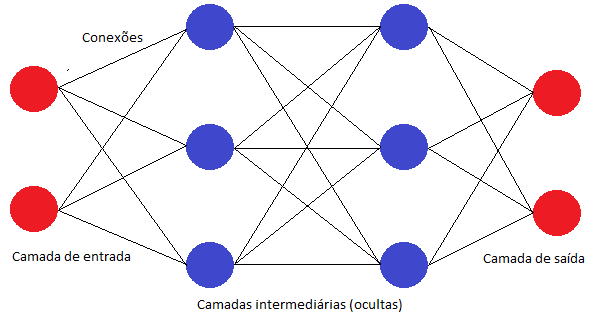
\includegraphics[scale=0.9]{figuras/rede-feedforward.png}
 	\fonte{Autor.}
 \end{figure}
 
 \subsubsection{Backpropagation}
 O backpropagation é um algoritmo de aprendizado supervisionado. Para se implementar esta técnica é necessário a existência de um “professor” que será responsável por estimular as entradas da rede  e comparar as saídas da mesma com o resultado esperado \cite{BRAGA}, veja a Figura 6. O processo se dá da seguinte forma: a rede é carregada com um conjunto de entradas, e através de uma configuração inicial de seus pesos, gera uma saída correspondente às entradas. A saída da RNA é comparada com a saída esperada e caso o erro seja superior ao limite definido pelo programador a rede reconfigura os pesos das suas sinapses, este processo se repete até que a rede obtenha uma saída satisfatória \cite{LANHELLAS}.

\begin{figure}[htb]
 \centering
 	\caption{Aprendizado supervisionado}
 	\label{fig:Aprendizado supervisionado}
 	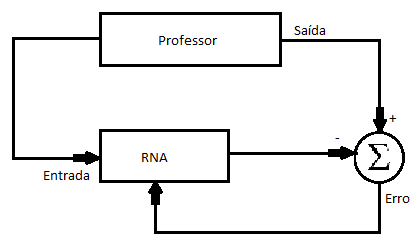
\includegraphics[scale=0.9]{figuras/aprendizado-supervizionado.png}
 	\fonte{Autor.}
 \end{figure}

% FALTA AJUSTAR \subsubsubsection{Exemplo subsubsubsection}